%!TEX encoding = UTF8
%!TEX root = 0-notes.tex

\chapter{Suites}

\dfn{Suite}{
	On appelle \emph{suite} une fonction $u$ réelle prenant des entiers naturels $n\in\N$.
	
	Le \emph{terme initial} de la suite est donné par $u(0)$.
	Le \emph{terme de rang $n$} de la suite est donné par $u(n)$.
}{dfn:suite}

\nt{
	Une suite est une liste de valeurs réelles $u(0), u(1), u(2), \dots$.
	On peut connaitre tous les termes d'une suite dès qu'elle est définie \emph{algébriquement}.
	C'est-à-dire, si $u(n) = \big(\text{expression en fonction de $n$}\big)$ pour tout $n\in\N$.
}

\ex{}{
	La suite donnée algébriquement par $u(n) = n-1$ pour tout $n\in\N$ est entièrement connue.
	Son terme initial est $u(0) = -1$, et son terme de rang $210$ est $u(210) = 209$.
}{ex:suite-alg}

\nt{
	Certaines suites peuvent être définies \emph{récursivement}.
	Le terme de rang $n$ dépendra des termes de rangs inférieurs.
}

\ex{}{
	Considérons la suite $u$ de terme initial $u(0) = 0$ et vérifiant, pour tout $n\in\N$,
		\[ u(n+1) = u(n) + 2. \]
	On lit « le terme de rang $n+1$ est égal au terme de rang $n$ plus 2 » ou, autrement dit, « pour passer d'un terme au suivant, il faut ajouter 2 ».
	Ainsi $u(1) = u(0) + 2 = 2, u(2) = 4, u(3) = 6, \dots$.
	
	Pour calculer $u(341)$, il faut, \emph{a priori} nécessairement calculer tous les termes de rang inférieur à $341$.
	Cependant, il semblerait $u(n) = 2n$ pour tout $n\in\N$, et donc qu'on ait immédiatement $u(341) = 682$.
}{ex:suite-rec}

\section{Suites arithmétiques}

\dfn{Suite arithmétique}{
	Une suite arithmétique $u$ est une suite vérifiant, pour tout $n\in\N$,
		\[ u(n+1) = u(n) + a, \]
	où $a\in\R$ est un nombre fixé qu'on appelle la \emph{raison}.
	
	On lit :
		\begin{center}
			« Pour passer d'un rang à l'autre, on ajoute la raison $a$. »
		\end{center}
}{dfn:suite-arithmetique}

\exe{}{
	Donner les 5 premiers termes de la suite arithmétique $u$ de raison 1 et de terme initial $u(0) = 0$.
	Faire une conjecture sur l'expression algébrique de $u(n)$ pour tout $n\in\N$.
}{exe:arithm1}{
	Pour passer d'un rang à l'autre, on ajoute la raison, ici $1$.
	Donc $u(1) = 0+1=1, u(2) = 2, u(3) = 3, u(4) = 4$.
	
	Il semblerait que $u(n) = n$ pour tout $n\in\N$.
}

\exe{}{
	Donner les 5 premiers termes de la suite arithmétique $v$ de raison 1 et de terme initial $v(0) = 3$.
	Faire une conjecture sur l'expression algébrique de $u(n)$.
}{exe:arithm2}{
	Pour passer d'un rang à l'autre, on ajoute la raison, ici $1$.
	Donc $v(1) = 3+1=4, v(2) = 5, v(3) = 6, v(4) = 7$.
	
	Il semblerait que $v(n) = n+1$ pour tout $n\in\N$.
}

\exe{}{
	Donner les 5 premiers termes de la suite arithmétique $w$ de raison -5 et de terme initial $w(0) = 5$.
	Faire une conjecture sur l'expression algébrique de $u(n)$.
}{exe:arithm3}{
	Pour passer d'un rang à l'autre, on ajoute la raison, ici $-5$.
	Donc $w(1) = 5-5=0, w(2) = -5, w(3) = -10, w(4) = -15$.
	
	Il semblerait que $w(n) = -5(n-1) = -5n + 5$ pour tout $n\in\N$.
}

\exe{}{
	Montrer que la suite $u$ dont les trois premiers termes sont $u(0) = 3, u(1) = 10, u(2) = 20$ ne peut pas être arithmétique.
}{exe:nonarithm}{
	Pour passer d'un terme à l'autre, on ajoute $7$ puis $10$.
	Si $u$ était arithmétique, on aurait ajouté la même quantité (sa raison). \Large\Lightning
}

\exe{}{
	Montrer que la suite $v$ telle que $v(41) = -10, v(42) = -20, v(44) = -30$ ne peut pas être arithmétique.
}{exe:nonarithm2}{
	Si $v$ était arithmétique, sa raison serait $-10$ car c'est ce qu'on ajoute pour passer du terme 41 au terme 42.
	Cependant, dans ce cas, on aurait $v(43) = -30$ et $v(44) = -40$, ce qui est contradictoire avec la donnée de l'exercice. \Large\Lightning
}

\exe{, difficulty=1}{
	Si une suite $w$ vérifie $w(10) = 1, w(11) = 3, w(12) = 5$, est-elle nécessairement arithmétique ?
}{exe:nonarithm3}{
	$w$ pourrait être arithmétique, auquel cas $w(n) = -9 + n$ pour tout $n\in\N$, mais ce n'est pas nécessairement le cas.
	On peut librement définir $w(13) = -100$ pour casser le caractère arithmétique de la suite. 
}

\thm{}{
	Soit $u$ une suite arithmétique de raison $a$ et de terme initial $u(0)$.
	Alors, pour tout $n\in\N$,
		\[ u(n) = u(0) + n\cdot a. \]
}{thm:suite-arithmetique}

\pf{}{
	Pour passer du terme initial au suivant, $u(1)$, on ajoute $a$.
	Pour arriver à celui d'après, on ajoute à nouveau $a$.
	Donc pour arriver au $n$-ième terme, on doit ajoute $n$ fois $a$ : $u(n) = u(0) + n\cdot a$.
	Ceci est vrai pour n'importe quel $n\in\N$.
}

\exe{}{
	Donner l'expression algébrique de la suite $u$ définie récursivement comme suit.
		\[ \begin{cases*} u(0) = 3, \\ u(n+1) = u(n) - 1 (n\in\N). \end{cases*}. \]
}{exe:arithm4}{
	$u$ est une suite arithmétique de terme initial $3$ et de raison $-1$.
	 D'après le théorème \ref{thm:suite-arithmetique}, $u(n) = 3-n$ pour tout $n\in\N$.
}

\exe{,difficulty=1}{
	On considère la série statistique $X=(0;1;2;\dots;19;20)$.
	Justifier sans calcul que la moyenne de $X$ est $10$.
	En déduire que $1+2+\cdots+19+20 = 210$.
}{exe:moyenne}{
	Par symétrie autour de $10$, la moyenne de $X$ vaut $10$ : toute valeur $10+k$ se compense avec $10-k$ pour $k=1, \dots, 10$, et la valeur $10$ seule est moyenne et n'a donc aucun impact.
	
	La formule de la moyenne donne $\dfrac{1+2+\cdots+19+20}{21} = 10$, d'où le résultat.
}

\thm{}{
	Pour tout $n\in\N$, on a l'égalité	
		\[ 0 + 1 + 2 + \cdots + n = \dfrac{n(n+1)}2. \]
}{thm:triangle}

\pf{}{
	Posons $S_n = 1 + 2 + \cdots + n$ pour $n\in\N$.
	
	\begin{multicols}{2}
	On considère le carré $(n+1) \times (n+1)$ ci-contre, découpé en $(n+1)^2$ carrés unités.
	
	En comptant les carrés sur chaque diagonale, on a 
		\[ S_n + (n+1) + S_n = (n+1)^2,\]
	ce qui conclut.
	
	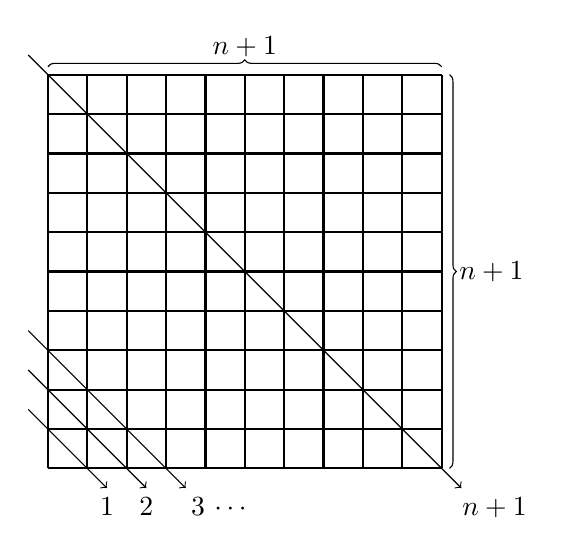
\begin{tikzpicture}[scale=0.5]
		\foreach \r in {0, ..., 10} {
			\draw[black,thick] (0,\r) -- (10,\r);
			\draw[black, thick] (\r,0) -- (\r, 10);
		}
		
		\draw[decoration={brace},decorate]
  			(0,10.2) -- node[above] {$n+1$} (10,10.2);
		\draw[decoration={brace, mirror},decorate]
  			(10.2,0) -- node[right] {$n+1$} (10.2,10);
  			
		\draw[->] (-0.5, 1.5) -- (1.5,-0.5) node[below] {$1$};
		\draw[->] (-0.5, 2.5) -- (2.5,-.5) node[below] {$2$};
		\draw[->] (-0.5, 3.5) -- (3.5,-.5) node[right=12pt, below] {$3$ $\cdots$};
		
		\draw[->] (-0.5, 10.5) -- (10.5,-.5) node[right=12pt, below] {$n+1$};
	
	\end{tikzpicture}
	\end{multicols}
}

\nomen{
	On appelle $S_n$ un \emph{nombre triangulaire} car il apparaît comme le nombre de carrés dans le triangle de la preuve du théorème \ref{thm:triangle}.
}

\notations{
	Au lieu de noter $S_n = 1 + 2 + \cdots + n$, on dit à l'oral « la somme des entiers de 1 à $n$ », car c'est plus court.
	On dit aussi « la somme des $k$, $k$ allant de 1 à $n$ », qu'on choisit de noter
		\[ S_n = 1 + 2 + \cdots + n = \text{« la somme des $k$, $k$ allant de 1 à $n$ »} = \sum_{k=1}^n k, \]
	où la lettre sigma majuscule $\Sigma$ désigne une somme.
	
	Plus généralement, on note
		\[ \sum_{k=a}^b u(k) = u(a) + u(a+1) + \cdots + u(b-1) + u(b). \]
}

\nt{
	Il est également possible d'indexer une somme sur un ensemble.
	Par exemple pour $E=\bigset{7; 11; 13 ; 17}$, 
		\begin{align*}
			\sum_{k\in E} k = 7+11+13+17 = 48, && \text{ et } && \sum_{k\in E} \dfrac1k = \dfrac17+\dfrac1{11}+\dfrac1{13}+\dfrac1{17} \approx 0,3695.
		\end{align*}
	
	Le deuxième théorème de Mertens implique que
		\[ \sum_{p \text{ premier}} \dfrac1p = \pinfty. \]
}

\exe{}{
	Donner les valeurs des sommes suivantes.
	\begin{multicols}{3}
		\begin{enumerate}[label=\roman*)]
		\item
		$\sum\limits_{k=1}^{10} 0$
		
		\item
		$\sum\limits_{k=1}^{10} 1$
		
		\item
		$\sum\limits_{k=0}^{10} 1$
		
		\item
		$\sum\limits_{k=-5}^{11} 1$
		
		\item
		$\sum\limits_{k=4}^{8} 2$
		
		\item
		$\sum\limits_{k=0}^{n} 1$
		
		\item
		$\sum\limits_{k=1}^{10} k$
		
		\item
		$\sum\limits_{k=1}^{20} k$
		
		\item
		$\sum\limits_{k=11}^{20} k$
		\end{enumerate}
	\end{multicols}
}{exe:sommes}{
	\begin{multicols}{3}
		\begin{enumerate}[label=\roman*)]
		\item
		$\sum\limits_{k=1}^{10} 0 = 0$.
		
		\item
		$\sum\limits_{k=1}^{10} 1 = 10$.
		
		\item
		$\sum\limits_{k=0}^{10} 1 = 11$.
		
		\item
		$\sum\limits_{k=-5}^{11} 1 = (11 + 5 + 1) = 17$.
		
		\item
		$\sum\limits_{k=4}^{8} 2 = 2(8-4+1) = 10$.
		
		\item
		$\sum\limits_{k=0}^{n} 1 = n$.
		
		\item
		$\sum\limits_{k=1}^{10} k = \dfrac{10(11)}2 = 55$.
		
		\item
		$\sum\limits_{k=1}^{20} k = \dfrac{20(21)}2 = 210$.
		
		\item
		$\sum\limits_{k=11}^{20} k = \sum\limits_{k=1}^{20} k - \sum\limits_{k=1}^{10} k = 210-55 = 155$.
		\end{enumerate}
	\end{multicols}
}

\thm{Linéarité de la somme}{
	Pour $c\in\R$ et $u, v,$ deux suites, on a 
		\[ \sum_{k=a}^{b} \bigl[ cu(k) + v(k) \bigr] =  c\sum_{k=a}^{b} u(k)+ \sum_{k=a}^{b}v(k). \]
}{thm:linéarité-somme}

\exe{,difficulty=1}{
	Démontrer le théorème \ref{thm:linéarité-somme}.
}{exe:linéarité-somme}{
	En explicitant la somme
		\[ \sum_{k=a}^{b} \bigl[ cu(k) + v(k) \bigr] = cu(a) + v(a) + cu(a+1) + v(a+1) + \cdots + cu(b) + v(b), \]
	on remarque qu'on peut regrouper les termes et factoriser par $c$ pour obtenir
		\[ \sum_{k=a}^{b} \bigl( cu(k) + v(k) \bigr) = c\bigl[u(a) + u(a+1) + \cdots + u(b)\bigr] + \bigl[v(a) + v(a+1) + \cdots + v(b)\bigr] = c\sum_{k=a}^{b} u(k)+ \sum_{k=a}^{b}v(k). \]
}

\lem{}{
	\[ \sum_{k=a}^{b} k = (b-a+1)\dfrac{a+b}2. \]
}{lem:somme-arithm}

\exe{,difficulty=2}{
	Démontrer le lemme \ref{lem:somme-arithm}.
}{exe:lem-somme-arithm}{
	On se ramène au cas $a=0$ pour utiliser le théorème \ref{thm:triangle}.
		\begin{align*}
			\sum_{k=a}^b k = \sum_{k=0}^b k - \sum_{k=0}^{a-1}
								= \dfrac{b(b+1)}2 - \dfrac{a(a-1)}2
								= \dfrac{(a+b)(b-a+1)}2.
		\end{align*}
}

\thm{Somme de série arithmétique}{
	Soit $u$ une suite arithmétique. Alors
		\begin{align*}
			\sum_{k=a}^b u(k) &= \text{(moyenne du premier et dernier terme) $\times$ (nombre de termes)} \\ &= \dfrac{u(a)+u(b)}2 \cdot (b-a+1).
		\end{align*}
}{thm:somme-arithm}

\exe{,difficulty=2}{
	Démontrer le théorème \ref{thm:somme-arithm}.
}{exe:somme-arithm}{
	Posons $u(n) = An +B$.
	Par linéarité de la somme, et d'après le lemme \ref{lem:somme-arithm},
		\begin{align*}
			\sum_{k=a}^b u(k) &= \sum_{k=a}^b \bigl[ Ak + B \bigr], \\
								&= A\sum_{k=a}^b k + B \sum_{k=a}^b 1, \\
								&= A \dfrac{(a+b)(b-a+1)}2 + B(b-a+1), \\
								&= (b-a+1) \dfrac{A(a+b) + 2B}2, \\
								&= (b-a+1) \dfrac{u(a) + u(b)}2.
		\end{align*}
}

\exe{}{
	Montrer que $\sum\limits_{k=a}^b u(k) = \sum\limits_{k=a-1}^{b-1} u(k+1)$.
}{exe:shiftk}{
	Expliciter la somme rend l'identité triviale.
}

\exe{, difficulty=2}{
	Posons $S_n = \sum\limits_{k=1}^{n+1} k^3$. 
	À l'aide de l'exercice \ref{exe:shiftk}, montrer qu'on a
		$S_n = \sum_{k=0}^{n} (k+1)^3.$
	En développant le cube et par linéarité de la somme, montrer que
		\[ S_n = S_n - (n+1)^3 + 3\sum_{k=0}^{n}k^2 + 3\sum_{k=0}^{n}k + n. \]
	En déduire la forme close
		\[ \sum_{k=0}^{n}k^2 = \dfrac{n(n+1)(2n+1)}6. \]
}{exe:somme-carres}{
	TODO
}

\exe{, difficulty=2}{
	En considérant la somme $S_n = \sum\limits_{k=1}^{n+1}k^4$, procéder comme à l'exercice \ref{exe:somme-carres} pour exprimer $\sum\limits_{k=1}^{n+1}k^3$ en fonction de $n$.
	En conclure que 
		\[ (1+2+\cdots+n)^2 = 1^3 + 2^3 + \dots + n^3 = \left[ \dfrac{n(n+1)}2 \right]^2. \]
}{exe:somme-cubes}{
	TODO
}

\exe{}{
	Au regard des exercices \ref{exe:somme-carres} et \ref{exe:somme-cubes}, déterminer combien d'opérations sont nécessaires pour calculer les sommes $1+2^2 + 3^2 + \cdots + n^2$ et $1+2^3 + 3^3 + \cdots + n^3$.
}{exe:complexité-somme}{
	Pour la première, il faut trois multiplications, une division, et deux additions, soit au total 6 opérations.
	Pour la seconde, il faut deux multiplications, une division, et une addition, soit au total 4 opérations.
}


\section{Suites géométriques}